This section is intended to make the developer understand the working of the Colletta backend, and to allow him or her to add functionalities  to the software package.
In order to fully understand the contents below, the developer must have a certain degree of familiarity with Java, the framework Spring Boot with his subframework Spring Data MongoDB, MongoDB and Maven. If that's not the case, we strongly recommend the reader to at least acquire some basic knowledge on the topics.

\subsection{Directory tree}

\begin{figure}[H]
\centering
\begin{forest}
  for tree={
    font=\ttfamily,
    grow'=0,
    child anchor=west,
    parent anchor=south,
    anchor=west,
    calign=first,
    inner xsep=7pt,
    edge path={
      \noexpand\path [draw, \forestoption{edge}]
      (!u.south west) +(7.5pt,0) |- (.child anchor) pic {folder} \forestoption{edge label};
    },
    before typesetting nodes={
      if n=1
        {insert before={[,phantom]}}
        {}
    },
    fit=band,
    before computing xy={l=15pt},
  }  
[Backend
	[src
		[main 
			[java
				[it
					[colletta
						[controller]
						[error]
						[exceptions]
						[library]
						[model
							[helper]
						]
						[repository]
						[security]
						[service]						
					]
				]
			]
			[resources]
		]	
		[test
			%[it
			%	[colletta
			%		[repository
			%			[config]
			%			[exercise]
			%			[phrase]
			%			[user]
			%		]
			%		[service
			%			[user]
			%		]
			%	]
			%]
		]				
	]
]
\end{forest}
\caption{Backend directory tree}
\label{fig:FrontDir}
\end{figure}

Each folder contains a specific set of files:
\begin{itemize}
\item  \textbf{controller:} classes that handle HTTP Request, marked with \textit{@RestController} Spring annotation;
\item  \textbf{error:} custom class for error handling;
\item  \textbf{exceptions:} custom class for exception handling;
\item  \textbf{library:} classes that connect the application to the PoS-tagging library;
\item  \textbf{model:} has the folder \textit{helper} which contains the transfer object (DTO), the other Model files are standard POJO objects that represent JSON objects store inside the database;
\item  \textbf{repository:} classes that encapsulates the set of objects persisted in a data store, in our case MongoDB, and the operations performed over them, providing a more object-oriented view of the persistence layer;
\item  \textbf{security:} classes that manages the security of the application through encryption and token management;
\item  \textbf{service:} classes that make up the logical business part of the application;
\item  \textbf{test:}  the tests that the application must pass to enter in a safe running state;
\item \textbf{resources:} contains the configuration file for connection to the database.
\end{itemize}

\subsubsection{Data and logic separation}
\begin{figure}[H]
\centering 
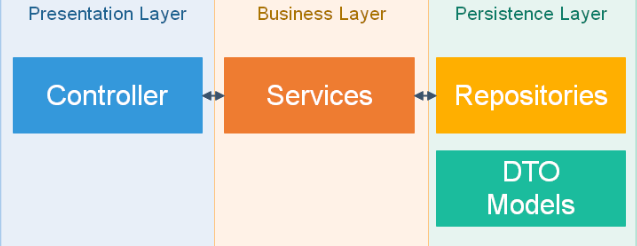
\includegraphics[scale=0.3]{uml/backendArchitecture.png} 
\caption{Data and logic separation}
\end{figure}

The design pattern used for the backend is: \textbf{Spring MVC}.
Respectively with the Controller, Service and Repository classes.
\\ 
To get more information about the architecture chosen for the backend, follow the link below: \href{https://docs.spring.io/spring/docs/current/spring-framework-reference/web.html}{Spring Web MVC}.

\subsubsection{Security}
The system was designed to secure client server communication so that only a user registered in the system can make calls which are then resolved by interacting with the database. 
In authentication, when the user successfully logs in using their credentials, a JSON Web Token will be returned, instead if the user has registered the token will be generated. Whenever the user wants to access a protected route or resource he/her must necessarily send his token that identifies him/her as a user correctly registered in the system. If this is not done the system will decline the request. 
The security system has been implemented so that the only requests that are authorized without token recognition are the login (\textit{/login}) and the registration (\textit{/sign-up}).\\
The system uses \textit{JWT tokens} for token authentication, more information is available at the link: \href{https://jwt.io/introduction/}{Introduction to JSON Web Tokens}. 
